\documentclass[11pt]{article}
\usepackage[T1]{fontenc}
\usepackage{graphicx}
\usepackage{amsmath}
\usepackage{amssymb}
\usepackage{fancyhdr}
\title{Środowisko Programisty - wzory skróconego mnożenia}
\author{Filip Bestfal}
\begin{document}
\maketitle
\newpage
\tableofcontents
\listoffigures
\listoftables
\newpage
\begin{center}
\section{Rozdział 1}
\label{sec:1. teoria}
\subsection{Podrozdział 1.1}
\end{center}
\begin{center}
Wzory skróconego mnożenia.
\end{center}
\begin{flushleft}
Wzór ogólny na wzory skróconego mnożenia wymyślił Isaac Newton, w postaci dwumianu Newtona.\footnote {Dwumian Newtona {${(x+y)^n} = {\sum_{i=1}^{n} }
{n \choose k} {a^{(n-k)}b^k}$}}\\
Wzory skróconego mnożenia to reguły rachunkowe pozwalające uprościć obliczenia na liczbach, wielomianach i elementach, dla których obowiązująprawa przemienności oraz łączności dodawania i mnożenia, a także rozdzielności mnożenia względem dodawania.\\
Do wzorów skróconego mnożenia zalicza się między innymi wzór na:
\end{flushleft}
\begin{flushleft}
\begin{eqnarray}
(a+b)^2 = a^2 + 2ab + b^2\\
(a-b)^2 = a^2 - 2ab + b^2\\
a^2 - b^2 = (a-b)(a+b)
\end{eqnarray}
\end{flushleft}
\begin{center}
\subsection{Podrozdział 1.2}
\end{center}
\begin{center}
Adnotację do podrozdziału 1.1
\end{center}
ad 1. Wzór przedstawia kwadrat sumy.\\
ad 2. Wzór przedstawia kwadrat różnicy.\\
ad 3. Wzór przedstawia różnicę kwadratów.
\newpage
\begin{center}
\section{Rozdział 2}
\subsection{Podrozdział 2.1}
\end{center}
\begin{center}
Wzory skróconego mnożenia trzeciej potęgi.
\end{center}
\begin{flushleft}
Ponadto istnieją również wzory skróconego mnożenia dla trzeciej potęgi.\\
A wyglądają one następująco :
\end{flushleft}
\begin{flushleft}
\begin{eqnarray}
(a+b)^3 = a^3 + 3a^2b + 3ab^2 + b^3\\
(a-b)^3 = a^3 - 3a^2b + 3ab^2 - b^3\\
a^3 - b^3 = (a-b)(a^2+ab+b^2)\\
a^3 + b^3 = (a+b)(a^2-ab+b^2)
\end{eqnarray}
\end{flushleft}
\begin{center}
\subsection{Podrozdział 2.2}
\end{center}
\begin{center}
Adnotację do podrozdziału 2.1
\end{center}
ad 4. Wzór przedstawia sześcian sumy.\\
ad 5. Wzór przedstawia sześcian różnicy.\\
ad 6. Wzór przedstawia różnicę sześcianów.\\
ad 7. Wzór przedstawia sumę sześcianów.\\
\newpage
\begin{center}
\section{Rozdział 3}
\label{sec:3. obrazki}
\subsection{Podrozdział 3.1}
\end{center}
\begin{center}
Obrazki przedstawiające graficznie wzory skróconego mnożenia.
\end{center}
\begin{figure}[h]
\begin{center}
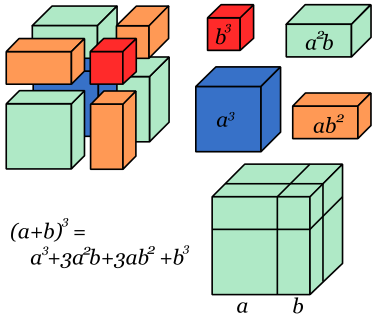
\includegraphics[width=5cm]{d.png}
\caption{Rysunek przestawiający graficznie wzór na sześcian sumy}
\end{center}
\end{figure}
\begin{figure}[h]
\begin{center}
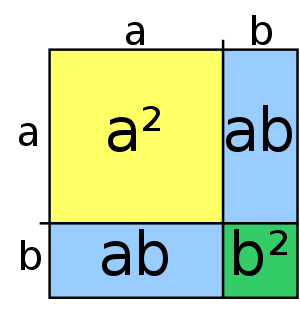
\includegraphics[width=5cm]{dd.png}
\caption{Rysunek przedstawiający graficznie kwadrat sumy}
\end{center}
\end{figure}
\newpage
\section{Wypunktowanie}
\begin{enumerate}
	\item Nie mam pomysłu na wypunktowanie
	\item ponieważ wykorzystałem wszystko
	\item co jest możliwe ze wzorów skróconego mnożenia
\end{enumerate}
\newpage
\section{Tabele}
\begin{table}[h]
\caption{ilosc wyrazow dla wyrazów o poszczególnych potęgach}
\begin{center}
\begin{tabular}{|c||l|l|l|l|}
\hline Potega & 1 & 2 & 3 & 4 \\ \hline \hline
Ilosc wyrazow & 1 & 3 & 5 & 6 \\ \hline
Liczby przy potegach & 1 & 1 2 1 & 1 4 6 4 1 & 1 5 10 10 5 1\\ \hline
\end{tabular}
\end{center}
\end{table}
\newpage
\section{Bibliografia}
\begin{thebibliography}{99}
\bibitem{pa}
\ref{sec:1. teoria} Pomoc ze strony :  https://matematyka.net/index.php/wzory/wzory-skroconego-mnozenia
\bibitem{pa}
\ref{sec:3. obrazki} Obrazki z arykułu wikipedii o wzorach skróconego mnożenia.
\end{thebibliography}
\end{document}